

\section {Вывод одномерных уравнений мелкой воды.}			% Заголовок
%\addcontentsline{toc}{chapter}{Вывод одномерных уравнений мелкой воды}	% Добавляем его в оглавление

\subsection {Вывод уравнения движения.}

Рассмотрим плавно изменяющееся движения жидкости, которое происходит в поле действия сил тяжести.

\begin{figure} [ht]
  \center
  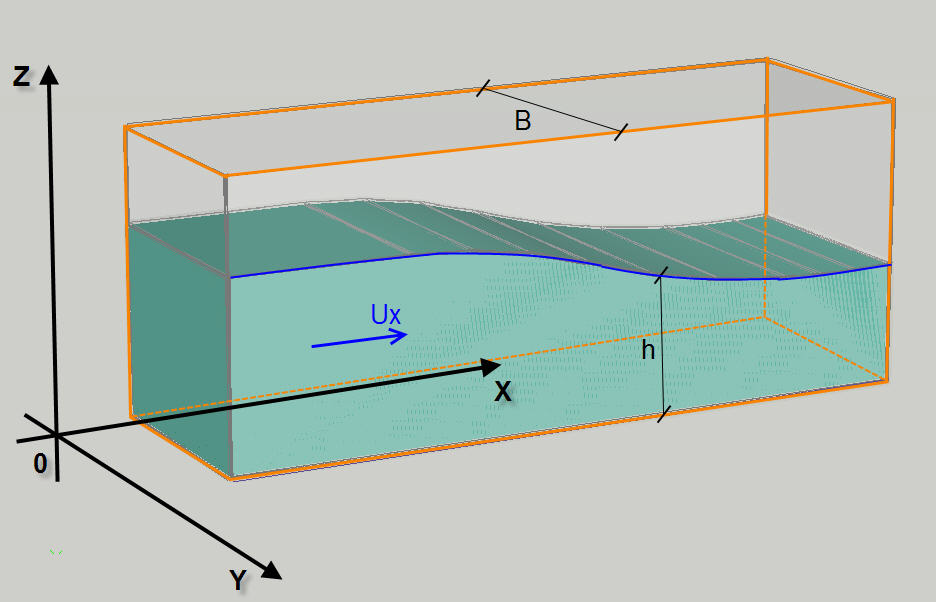
\includegraphics [scale = 0.5] {image1}
  \caption{К выводу уравнения движения.}
  \label{image1}
\end{figure}

Поскольку движение жидкости плавноизменяющееся живые сечения можно считать плоскими, а распределение давления в этих сечениях принять гидростатическим.
Таким образом, для величины давления в каждой точке такого потока должны выполняться уравнения равновесия покоящейся жидкости:

\begin{equation}
\left\{
  \label{eq_EulerStat}
{\setlength\arraycolsep{2pt}
  \begin{array}{rl}
     \vspace{5pt}
     \displaystyle X - \frac{1}{\rho} \frac{ \partial p}{ \partial x} = & 0  \\
     \vspace{5pt}
     \displaystyle Y - \frac{1}{\rho} \frac{ \partial p}{ \partial y} = & 0  \\
     \displaystyle Z - \frac{1}{\rho} \frac{ \partial p}{ \partial z} = & 0 \ ,
  \end{array}
}
\right.
\end{equation}

\noindent где $X,\ Y,\ Z$ -- проекции единичных массовых сил, действующих на рассматриваемую жидкость; 

$\rho$ -- плотность рассматриваемой жидкости; 

$p$ -- давление. \\

Так как давление распределено статически, величина давления в любом сечении потока зависит только от глубины (\ref{eq_p1}, \ref{eq_p2}), то при перемещении вдоль оси OX рассматриваемого потока давление будет изменяться со скоростью, зависящей только от приращения глубин. Определим величину этой скорости изменения давления, для этого рассмотрим поток жидкости с положительным уклоном свободной поверхности (рис.\ref{image2}). 

\newpage

\begin{figure} [ht]
  \center
  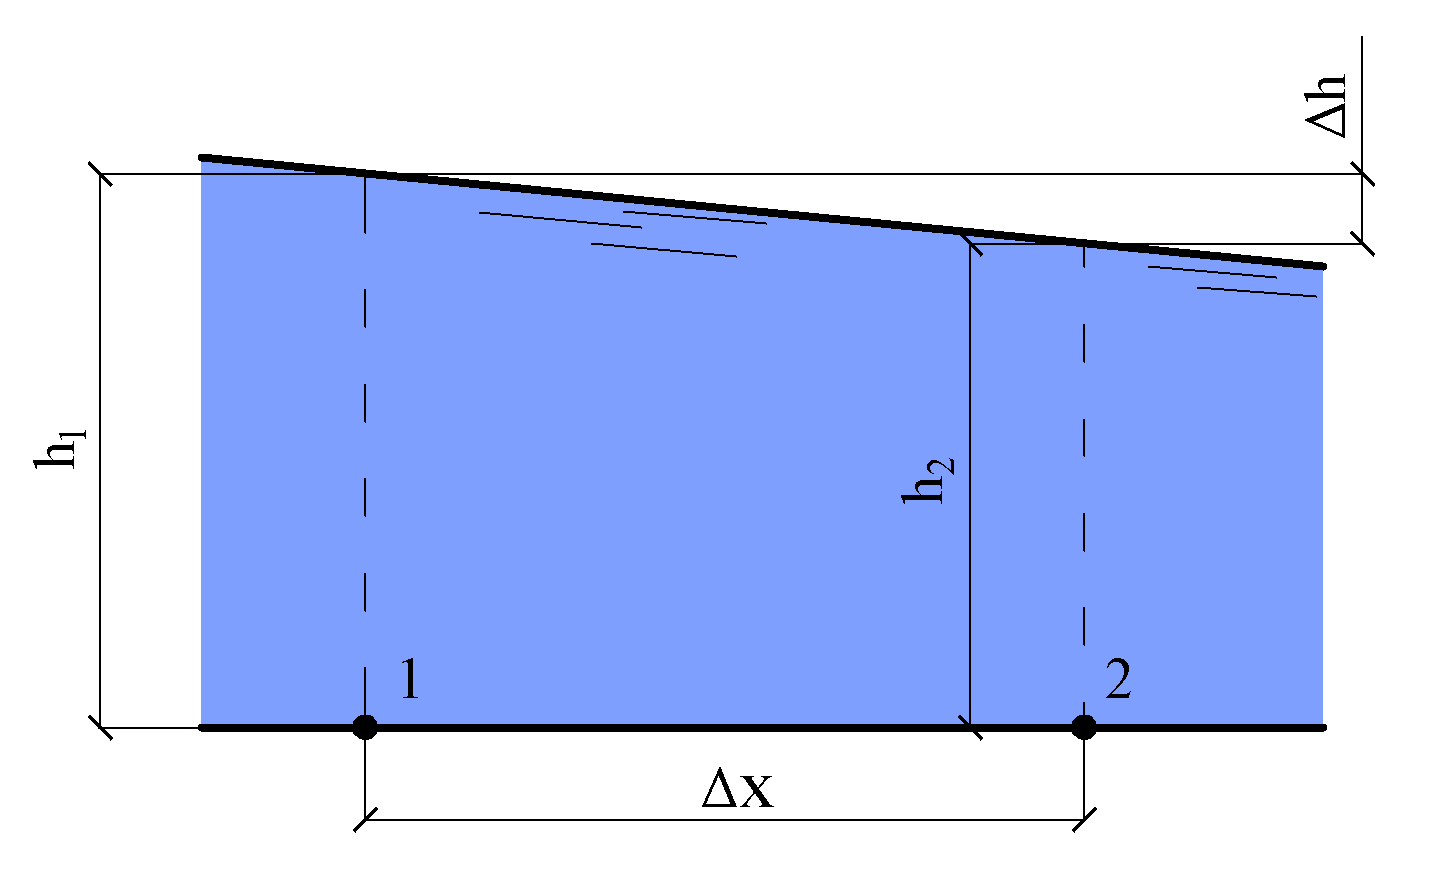
\includegraphics [scale = 0.8] {image2}
  \caption{К определению скорости изменения давления.}
  \label{image2}
\end{figure}

Поскольку давление в потоке распределено гидростатически, величина давления в точках 1 и 2 этого потока определяется по основному уравнению гидростатики:

\begin{equation}
  \label{eq_p1}
  p_1 = p_0 + \rho g h_1
\end{equation}

\begin{equation}
  \label{eq_p2}
  p_2 = p_0 + \rho g h_2
\end{equation}

При перемещении из точки 1 в точку 2, которые находятся на расстоянии $ \Delta x $ друг от друга, давление изменится на величину:

$$
  \Delta p = ( p_0 + \rho g h_2 ) - ( p_0 + \rho g h_1 ) = \rho g (h_2- h_1) = \rho g \Delta h \ ,
$$

\noindent где

$$
  \displaystyle \Delta h = h_2- h_1 = \frac{\partial h}{\partial x} \Delta x \ ,
$$

\noindent откуда

$$
  \displaystyle \Delta p = \rho g \frac{\partial h}{\partial x} \Delta x 
$$

И скорость изменения давления при перемещении вдоль оси OX:

\begin{equation}
  \label{eq_deltap_po_x}
  \displaystyle \frac{\partial p}{\partial p} = \frac{\Delta p} {\Delta x} = \rho g \frac{\partial h}{\partial x} \ ,
\end{equation}

\vspace{0.5cm}

Теперь запишем для рассматриваемого потока (рис.\ref{image1}) уравнения движения.

\begin{equation}
\left\{
  \label{eq_EulerDyn}
{\setlength\arraycolsep{2pt}
  \begin{array}{rl}
     \vspace{5pt}
     \displaystyle X' - \frac{1}{\rho} \frac{ \partial p}{ \partial x} - \frac{d U_x}{d t} = & 0  \\
     \vspace{5pt}
     \displaystyle Y' - \frac{1}{\rho} \frac{ \partial p}{ \partial y} - \frac{d U_y}{d t} = & 0  \\
     \displaystyle Z' - \frac{1}{\rho} \frac{ \partial p}{ \partial z} - \frac{d U_z}{d t} = & 0 \ ,
  \end{array}
}
\right.
\end{equation}

\noindent где $X', Y', Z'$ -- проекции единичных массовых сил, действующих в движущейся жидкости, причём:

\vspace{0.2cm}

$ \displaystyle X' = \frac{ -F_{friction} }{g} \neq X $, поскольку силы трения $ F_{friction} $ проявляются только в движении; 

$ Y' = 0 $;

$ Z' = Z = -g $. \\ 


В связи с тем, что для этого потока также справедлива система (\ref{eq_EulerStat}) то, так как $ Z = Z' $:

$$ 
  \displaystyle Z' - \frac{1}{\rho} \frac{\partial p}{\partial z} = 0
$$

После подстановки этого условия статического распределения давления в систему (\ref{eq_EulerDyn}) её третье уравнение (проекция на OZ) будет иметь вид:

$$
  \displaystyle \frac{d U_z}{d t} = 0
$$

Для перехода к двумерной задаче положим координату $ y = 0 $, исключив из рассмотрения второе уравнение системы (\ref{eq_EulerDyn}), при этом подразумевая, что ширина потока вовсе не нулевая, однако параметры, характеризующие состояние потока в этом направлении постоянны для каждого момента времени:

\begin{equation}
   \label{eq_uslov2d}
   \displaystyle \frac{\partial p}{\partial y} = 0 ;\  \frac{\partial U_x}{\partial y} = 0 ;\  \frac{\partial U_y}{\partial y} = 0 ;\  \frac{\partial U_z}{\partial y} = 0 .
\end{equation}

И, соответственно, система уравнений (\ref{eq_EulerDyn}) примет вид:

$$
   \left\{
{\setlength\arraycolsep{2pt}
  \begin{array}{rl}
     \vspace{5pt}
    & \displaystyle  X' - \frac{1}{\rho} \frac{ \partial p}{ \partial x} - \frac{d U_x}{d t} = 0  \\
    & \displaystyle  \frac{d U_z}{d t} = 0 
  \end{array}
}
\right.
$$

\vspace{1cm}

Рассмотрим первое уравнение получившейся системы:

\begin{equation}
  \label{eq_uravnDvi1}
  \displaystyle \frac{1}{\rho} \frac{ \partial p}{ \partial x} + \frac{d U_x}{d t} - X' = 0 \ ,
\end{equation}

\noindent где $ X' = -\frac{ F_{friction} }{g} $, $  \frac{\partial p}{\partial p} = \rho g \frac{\partial h}{\partial x} $ в соответствии с (\ref{eq_deltap_po_x}), а $ \frac{d U_x}{d t} $ является субстанциональной производной:

$$
  \displaystyle \frac{d U_x}{d t} = \frac{\partial U_x}{\partial t} + \frac{\partial U_x}{\partial x} U_x + \frac{\partial U_x}{\partial y} U_y + \frac{\partial U_x}{\partial z} U_z
$$

Из выражения (\ref{eq_uslov2d}) $ \frac{\partial U_x}{\partial y} = 0 $. Величину проекции скорости в направлении ОХ примем постоянной и равной средней на вертикали скорости $ U_x = U $ ($ \frac{\partial U_x}{\partial z} = 0 $), и, таким образом, от двумерной задачи перейдём к одномерной. Тогда:

\begin{equation}
  \label{eq_substU}
  \displaystyle \frac{d U_x}{d t} = \frac{\partial U_x}{\partial t} + \frac{\partial U_x}{\partial x} U_x = \frac{\partial U}{\partial t} + \frac{\partial U}{\partial x} U 
\end{equation}

С учётом вышесказанного (\ref{eq_deltap_po_x}, \ref{eq_substU}) перепишем выражение (\ref{eq_uravnDvi1}).

$$
  \displaystyle \frac{1}{\rho} \left( \rho g \frac{ \partial h}{ \partial x} \right) + \frac{\partial U}{\partial t} + \frac{\partial U}{\partial x} U + \frac{F_{friction}}{\rho} = 0
$$

\begin{equation}
  \label{eq_uravnDvi2}
\displaystyle g \frac{ \partial h}{ \partial x} + \frac{\partial U}{\partial t} + U \frac{\partial U}{\partial x} + \frac{F_{friction}}{\rho} = 0
\end{equation}

\vspace{1cm}

Величина силы трения $ F_{friction} $ в поледнем выражении может быть определена по формуле Шези:

$$
  U = C\sqrt{RI} \ ,
$$

\noindent где $ U $ -- средняя скорость в рассматриваемом сечении; 

$ R $ -- гидравлический радиус; 

$ C $ -- коэффициент Шези; 

$ I = \frac{h_f} {l} $ -- гидравлический уклон; 

$ h_f $ -- потери полного напора на участке потока длиной $ l $. \\

Поскольку потери напора по физическому смыслу представляют собой изменение полной удельной энергии потока, отнесённые к единице веса рассматриваемой жидкости, то, учитывая что изменение полной удельной энергии потока происходит только засчёт работы сил трения $ A = F_{friction} \cdot l $ (равномерное движение):

$$
  \displaystyle h_f = \frac{f_{friction} \cdot l}{G} \ ,
$$

\noindent где $ G = \rho g 1 $ -- вес единичного объёма рассматриваемой жидкости. \\

Итак, уравнение Шези:

$$
  \displaystyle U = C \sqrt{R \frac{F_{friction} \cdot l}{l \rho g} }
$$

Откуда:

\begin{equation}
  \label{eq_Ffric}
  \displaystyle F_{friction} = \frac{U^2}{C^2 R} \cdot \rho g
\end{equation}

После подстановки полученного выражения для $ F_{friction} $ в выражение (\ref{eq_uravnDvi2}) получим окончательный выд уравнения движения мелкой воды.

\begin{equation}
  \label{eq_uravnDvi}
\displaystyle \frac{\partial U}{\partial t} + U \frac{\partial U}{\partial x} + g \frac{ \partial h}{ \partial x} + g \frac{U^2}{C^2 R} = 0
\end{equation}

\vspace{0.5cm}

Для того чтобы описать движение потока воды в одномерной постановке, уравнения (\ref{eq_uravnDvi}) недостаточно, необходимо дополнить его уравнением неразрывности.

\newpage

%--------------------------------------------------------------------------------------------------------------------
% вывод уравнения неразрывности
%--------------------------------------------------------------------------------------------------------------------

\subsection {Вывод уравнения неразрывности.}

Для вывода уравнения неразрывности рассмотрим неподвижный прямоугольный параллелепипед, сквозь который протекает поток жидкости.

\begin{figure} [ht]
  \center
  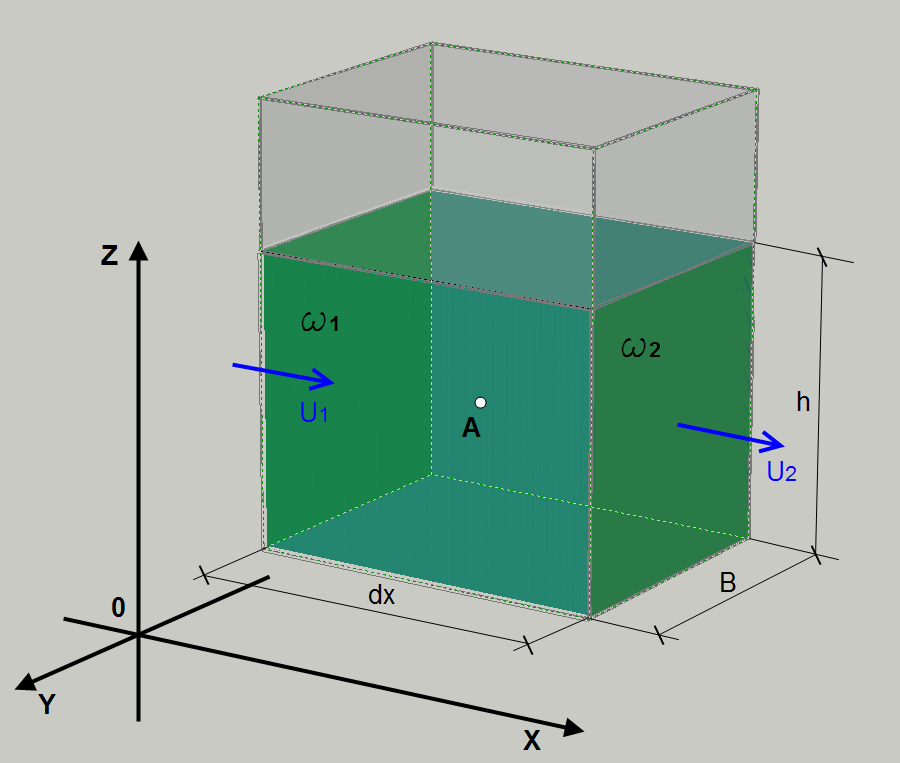
\includegraphics [scale = 0.4] {image3}
  \caption{К выводу уравнения неразрывности.}
  \label{img_image3}
\end{figure}

Рассматриваемый параллелепипед имеет длину $ d x $ вдоль потока жидкости, ширину $ B $ поперёк потока.

Поток жидкости движется вдоль оси OX. Скорости потока в пределах поперечных сечений $ \omega_1 $ и $ \omega_2 $ принимаются постоянными в пределах этих сечений (средние скорости).

Предположим, что в течение некоторого промежутка времени расход потока жидкости неравномерно распределён вдоль оси OX. Такое предположение можно представить при условии, что поверхность жидкости в пределах параллелепипеда повышается вдоль оси ОХ\footnote{На самом деле поверхность в пределах параллелепипеда всегда параллельна плоскости XY, предположение о её уклоне вводится лишь для установки логической связи между изменением расхода вдоль ОХ и положением уровня жидкости.} (т.е. в сечение $ \omega_2 $ находится гребень продольной волны потока жидкости). В течение рассматриваемого промежутка времени вследствие действия сил тяжести поверхность жидкости будет стремиться к горизонтальной, а следовательно, расход жидкости, проходящий через сечение $ \omega_2 $ будет больше, чем расход через сечение $ \omega_1 $.

При таком изменении расхода (увеличении его вдоль ОХ) поверхность жидкость в параллелепипеде будет понижаться, причём вследствие малости величины $ dx $ можно считать, что положение свободной поверхности жидкости в параллелепипеде во всех точках (в плоскости XY) за промежуток времени $ dt $ изменится на одинаковую величину $ dh $.

Итак, за промежуток времени $ dt $ объём жидкости в параллелепипеде изменится. Поскольку уровень воды уменьшается со скоростью $ - \frac{dh}{dt} $, то приращение объёма параллелепипеда:

\begin{equation}
  \label{dvhparall}
  \displaystyle dV_h = -\frac{\partial h}{\partial t} dt B dx
\end{equation}

Это приращение объёма происходит засчёт того, что расход жидкости, поступающей в параллелепипед через сечение $ \omega_1 $ не равен расходу жидкости, выходящей из параллелепипеда через сечение $ \omega_2 $. То есть можно написать также:

$$
  dV_Q = \delta Q \cdot dt = (Q_2 - Q_1) dt
$$

Если предположить, что расход в центре параллелепипеда (в точке А) равен $ Q_A $ тогда расход, проходящий через сечение $ \omega_1 $:

$$
  \displaystyle Q_1 = Q_A - \frac{\partial Q}{\partial x} \frac{dx}{2} = Q_A - \frac{\partial (\omega_1 U_1)}{\partial x} \frac{dx}{2}
$$

Расход, проходящий через сечение $ \omega_2 $:

$$
  \displaystyle Q_2 = Q_A + \frac{\partial Q}{\partial x} \frac{dx}{2} = Q_A + \frac{\partial (\omega_2 U_2)}{\partial x} \frac{dx}{2}
$$

Тогда приращение объёма жидкости в параллелепипеде, обусловленное неравномерностью расхода вдоль ОХ:

$$
  \displaystyle dV_Q = \frac{\partial (\omega U)}{\partial x} dx dt
$$

Учитывая, что $ \omega = B \cdot h $, а также применяя правило дифференцирования произведения можно написать:

$$
  \displaystyle dV_Q = \frac{\partial (h \cdot U)}{\partial x} B dx dt



  \displaystyle dV_Q = \left( U \frac{\partial h}{\partial x} + h \frac{\partial U}{\partial x} \right)   B dx dt
$$

Поскольку $ dV_h = dV_Q $,

$$
  \displaystyle -\frac{\partial h}{\partial t} dt B dx = \left( U \frac{\partial h}{\partial x} + h \frac{\partial U}{\partial x} \right)   B dx dt
$$ 

И уравнение неразрывности в одномерной постановке задачи примен вид:

\begin{equation}
  \label{eq_urNerazr}
  \displaystyle \frac{\partial h}{\partial t} + U \frac{\partial h}{\partial x} + h \frac{\partial U}{\partial x} = 0
\end{equation}

\vspace{1.5cm}

Итак, система одномерных уравнений, позволяющих описать движение потока жидкости имеет вид:

\begin{equation}
  \label{eq_urMelkovod}
     \left\{
{\setlength\arraycolsep{2pt}
  \begin{array}{rl}
     \vspace{5pt}
    & \displaystyle \frac{\partial U}{\partial t} + U \frac{\partial U}{\partial x} + g \frac{ \partial h}{ \partial x} + g \frac{U^2}{C^2 R} = 0  \\
    & \displaystyle \frac{\partial h}{\partial t} + U \frac{\partial h}{\partial x} + h \frac{\partial U}{\partial x} = 0
  \end{array}
}
\right.
  
\end{equation}


















